\section{Power}
In order to provide power to everything, we can utilize the following current feedback Opamp-based virtual ground driver, provided from \cite{TangentSoft}. It provides up to 250mA of current and creates a virtual ground, allowing negative voltages, something we need for the HMC694LPE Variable Gain Amplifier. 

\begin{figure}[H]
    \centering
    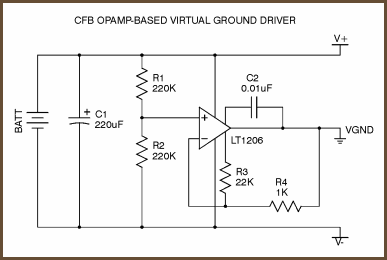
\includegraphics[width = 0.6\textwidth]{Images/cfb-opa.png}
    \caption{Current Feedback Operational Amplifier Virtual Ground Driver}
    \label{fig:cfbopa}
\end{figure}

We must also verify that this power supply can provide the maximum current required by the circuit. We can check all the essential components in this system. All information in the following table has been found from their respective datasheets:


\begin{tabular}{||c|c|c|c||}
    \cline{1-2}
    Manufacturer & Component & Datasheet Reference & Max. Current Draw\\
    \hline \hline
     Z-Communications & DRO10000A & Power Supply Req.: Supply Current & 26 mA \\
    \hline
     Analog Devices & HMC694LPE & Total Supply Current & 175 mA \\
    \hline
     Texas Instruments & OPA 207 & Short Circuit Current & 40 mA \\
    \hline
     Mini-Circuits & YAT-30A+ & N/A & 0mA \\
    \cline{3-4}
\end{tabular}

Summing the four main power intensive components in this circuit results in 241 mA of maximum current draw. This is cutting it a little close to the maximum current that the power supply can provide, but since it still is within spec, we will assume this power supply to work just fine.

\paragraph{YAT-30A+}
Note: The YAT-30A+ is specified in the datasheet that it can take signals up to 1W. The input AM wave reaches up to 20dBm, satisfying this condition. Therefore, it requires no current from the power supply.